\chapter{p3 = 5 (3 graphs)}
\newpage\begin{figure}
  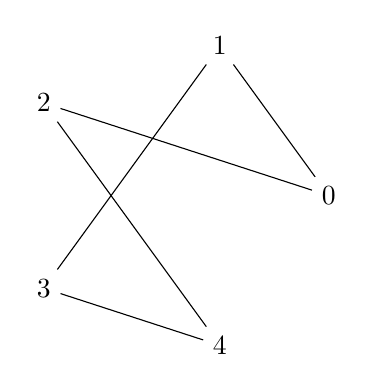
\begin{tikzpicture}
      \draw
        (0.0:2) node (0){0}
        (72.0:2) node (1){1}
        (144.0:2) node (2){2}
        (216.0:2) node (3){3}
        (288.0:2) node (4){4};
      \begin{scope}[-]
        \draw (0) to (1);
        \draw (0) to (2);
        \draw (1) to (3);
        \draw (2) to (4);
        \draw (3) to (4);
      \end{scope}
    \end{tikzpicture}
\end{figure}
\begin{itemize}
\item signature: 1100010011
\item g: Graph with 5 nodes and 5 edges
\item order: 5
\item size: 5
\item max degree: 2
\item degrees: 2,2,2,2,2
\item is tree: 0
\item is bipartite: 0
\item has bridge: 0
\item is chordal: 0
\item is complete: 0
\item min cycle basis weight: 5
\item min cycle basis size: 1
\item diameter: 2
\item radius: 2
\item is eulerian: 1
\item is planar: 1
\item number of faces: 2
\item is regular: 1
\item p3: 5
\item p4: 5
\item property hash: 8181b82b8bf3814ab44ea7a99a158bcd5a2bfb337c88b164c04b7f44288d2ac4
\end{itemize}
\newpage
\begin{figure}
  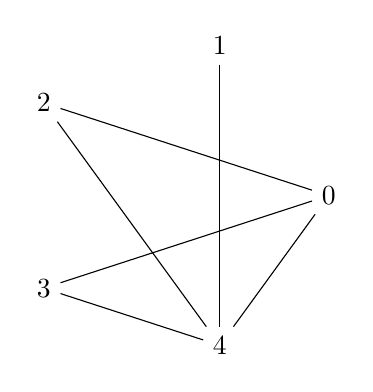
\begin{tikzpicture}
      \draw
        (0.0:2) node (0){0}
        (72.0:2) node (1){1}
        (144.0:2) node (2){2}
        (216.0:2) node (3){3}
        (288.0:2) node (4){4};
      \begin{scope}[-]
        \draw (0) to (2);
        \draw (0) to (3);
        \draw (0) to (4);
        \draw (1) to (4);
        \draw (2) to (4);
        \draw (3) to (4);
      \end{scope}
    \end{tikzpicture}
\end{figure}
\begin{itemize}
\item signature: 0111001011
\item g: Graph with 5 nodes and 6 edges
\item order: 5
\item size: 6
\item max degree: 4
\item degrees: 1,2,2,3,4
\item is tree: 0
\item is bipartite: 0
\item has bridge: 1
\item is chordal: 1
\item is complete: 0
\item min cycle basis weight: 6
\item min cycle basis size: 2
\item diameter: 2
\item radius: 1
\item is eulerian: 0
\item is planar: 1
\item number of faces: 3
\item is regular: 0
\item p3: 5
\item p4: None
\item property hash: 77fd5212c5ed261fbbf013cf4b1aa9ae52986d56c23b80af3530e2440d8a2dad
\end{itemize}
\newpage
\begin{figure}
  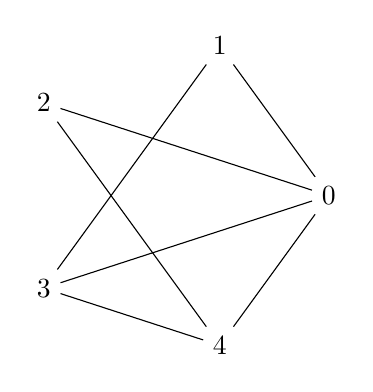
\begin{tikzpicture}
      \draw
        (0.0:2) node (0){0}
        (72.0:2) node (1){1}
        (144.0:2) node (2){2}
        (216.0:2) node (3){3}
        (288.0:2) node (4){4};
      \begin{scope}[-]
        \draw (0) to (1);
        \draw (0) to (2);
        \draw (0) to (3);
        \draw (0) to (4);
        \draw (1) to (3);
        \draw (2) to (4);
        \draw (3) to (4);
      \end{scope}
    \end{tikzpicture}
\end{figure}
\begin{itemize}
\item signature: 1111010011
\item g: Graph with 5 nodes and 7 edges
\item order: 5
\item size: 7
\item max degree: 4
\item degrees: 2,2,3,3,4
\item is tree: 0
\item is bipartite: 0
\item has bridge: 0
\item is chordal: 1
\item is complete: 0
\item min cycle basis weight: 9
\item min cycle basis size: 3
\item diameter: 2
\item radius: 1
\item is eulerian: 0
\item is planar: 1
\item number of faces: 4
\item is regular: 0
\item p3: 5
\item p4: None
\item property hash: 1115f1191acd1df002e505ac908438791dac8e8ea8c0cb82752f8fc08a6b1937
\end{itemize}
\newpage
